%------------------------------------------------------------------------------------------------------------
\section{Data structures} \label{sec:DataStructures}
%------------------------------------------------------------------------------------------------------------

An overview of the data structures implemented in the AMIDST toolbox is illustrated in Figure \ref{Figure:ToolboxDataStructures}. These data structures basically define the main components that will be used afterwards for implementing the AMIDST learning and inference algorithms. 

\vspace{-0.1in}

\begin{figure}[ht!]
\begin{center}
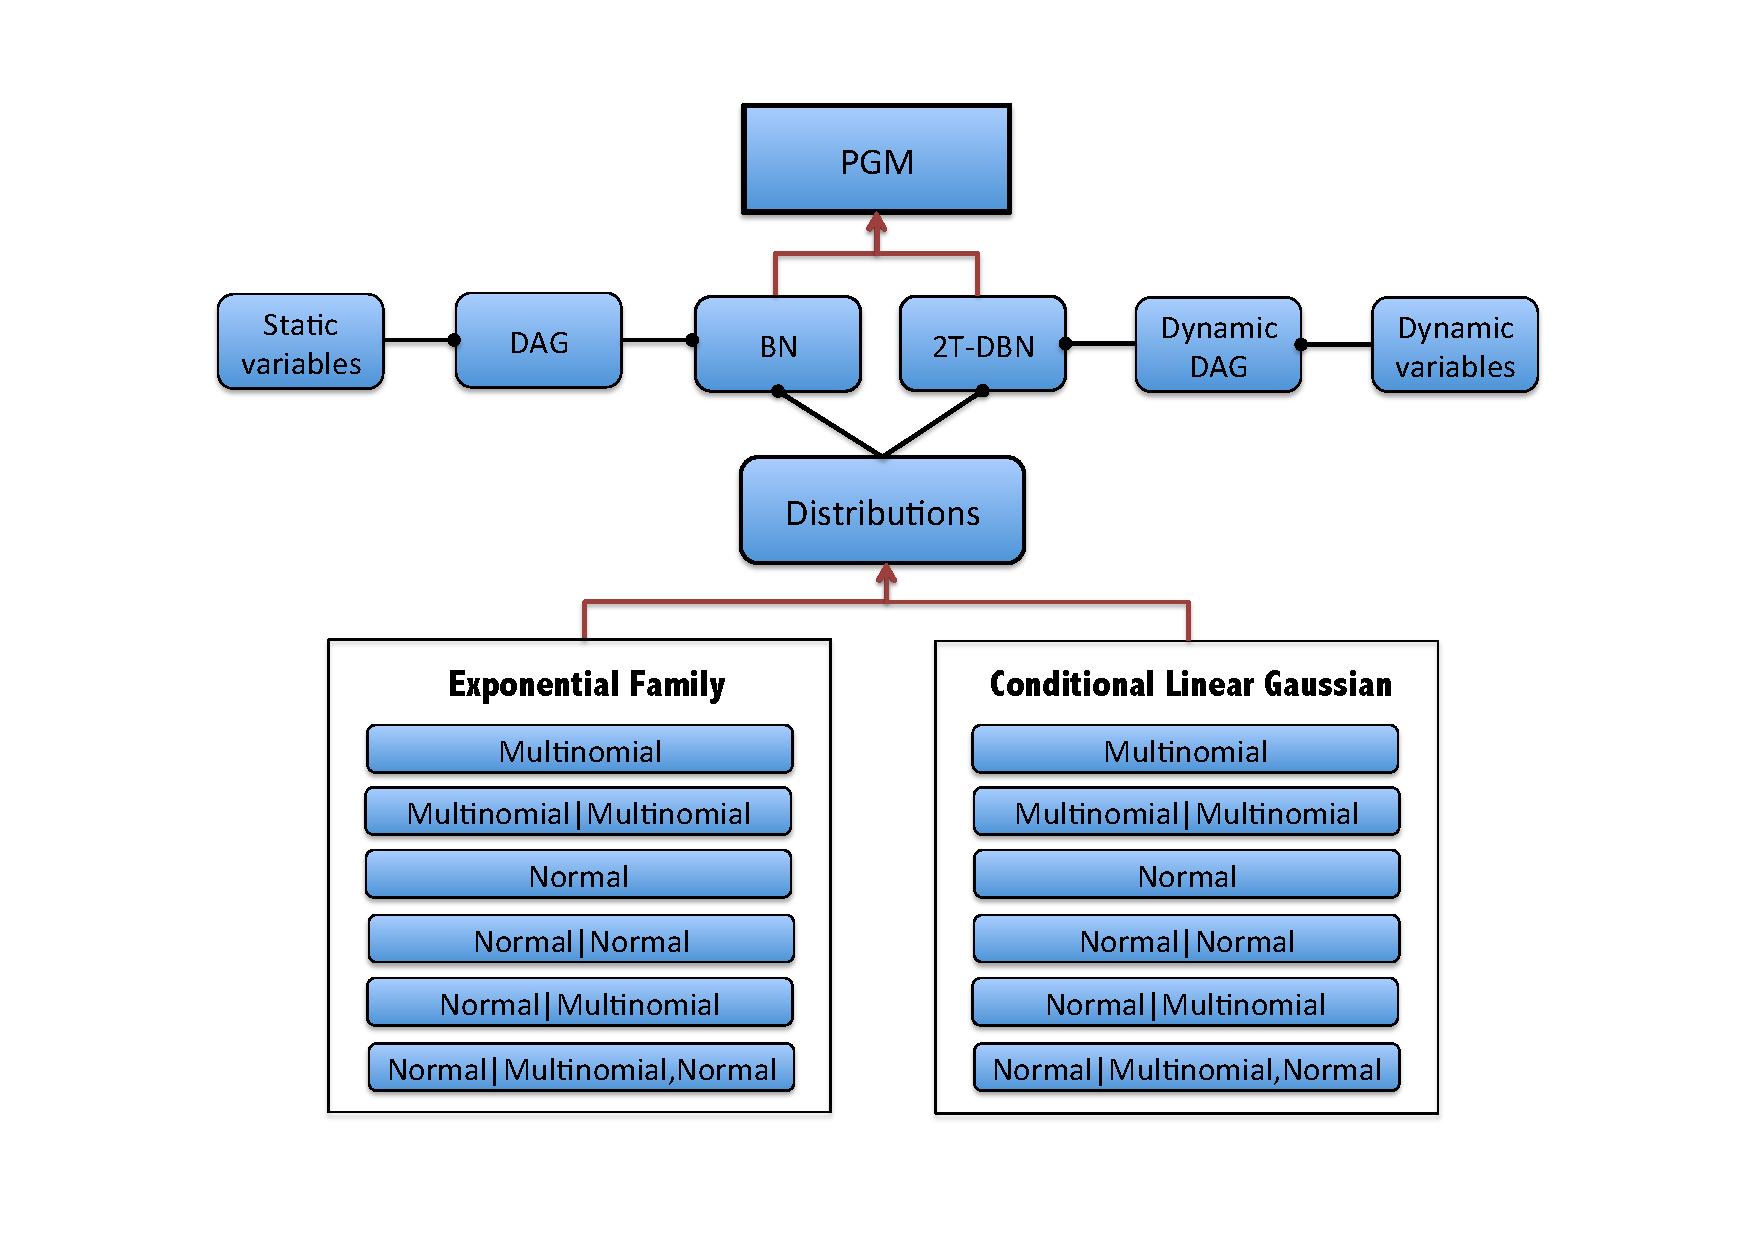
\includegraphics[width=\linewidth]{./figures/DataStructure}
\vspace{-0.5in}
\caption{\label{Figure:ToolboxDataStructures} Illustration of AMIDST toolbox data structure components. Nomenclature: The boxes in the
      figure represent software components (sets, possibly singletons, of classes), a rounded-arc going from $X$ to $Y$ indicates that $Y$ 'uses/references' $X$, and an arc with an arrow from $X$ to $Y$ implies inheritance.}
\end{center}
\end{figure}

In what follows, we briefly define each component and how it can be used in AMIDST toolbox through providing some code excerpts. 


%------------------------------------------------------------------------------------------------------------
\subsection{Probabilistic graphical model (\comp{PGM})}
%------------------------------------------------------------------------------------------------------------

 A probabilistic graphical model is a framework consisting of two parts: a qualitative component in the form of a graphical model encoding conditional independence assertions about the domain being modelled as well as a quantitative component consisting of a collection of local probability distributions adhering to the independence properties specified in the graph- ical model. Collectively, the two components provide a compact representation of the joint probability distribution over the domain being modelled.
 
In the AMIDST toolbox, we currently focus on two specific instantiations of PGMs, namely, a static Bayesian network (\comp{BN} component) and a two time-slice dynamic Bayesian network (\comp{2T-DBN}). 
 

%------------------------------------------------------------------------------------------------------------
\subsection{Static variables}
%------------------------------------------------------------------------------------------------------------

Static variables consist of a list of objects of type \texttt{Variable} that are used later to build a static Bayesian network. Each static variable is characterized by its name, ID, the state space type, the distribution type (i.e., multinomial or normal), as well as if it is observed or not. 

Note that observed static variables are initialised using the list of attributes (that are already parsed from the dataset or specified by the user), then hidden static variables are afterwards specified by the user.

\begin{table}[H]
\begin{tabular}{l} \\ \hline

        \texttt{StaticVariables variables = new StaticVariables(data.getAttributes());}\\

        \texttt{Variable A = variables.getVariableByName("A");}\\
        \texttt{Variable B = variables.getVariableByName("B");}\\
        \texttt{Variable C = variables.getVariableByName("C");}\\\\

        \texttt{VariableBuilder variableBuilder = new VariableBuilder();}\\
        \texttt{variableBuilder.setName("HiddenVar");}\\
        \texttt{variableBuilder.setObservable(false);}\\
        \texttt{variableBuilder.setStateSpace(new }\\  \texttt{~~~~~~MultinomialStateSpace(Arrays.asList("TRUE","FALSE")));}\\
        \texttt{variableBuilder.setDistributionType(DistType.MULTINOMIAL);}\\
        \texttt{Variable hidden = variables.addHiddenVariable(variableBuilder);}\\ \hline 

\end{tabular}
\end{table}


%------------------------------------------------------------------------------------------------------------
\subsection{Directed acyclic graph (\comp{DAG})}
%------------------------------------------------------------------------------------------------------------

A directed acyclic graph (\comp{DAG}) defines the Bayesian network graphical structure over a list of \comp{Static variables}, such that he dependence relationships between the variables are established through the definition of the parent set for each variable. 

\begin{table}[H]
\begin{tabular}{l} \\ \hline

        \texttt{WekaDataFileReader reader = new}\\
         \texttt{~~~~~~WekaDataFileReader("data/dataWeka/contact-lenses.arff");}\\

        \texttt{StaticVariables variables = new StaticVariables(reader.getAttributes());}\\
        \texttt{DAG dag = new DAG(variables);}\\\\

        \texttt{StaticVariables variables = dag.getStaticVariables();}\\
        \texttt{Variable A = variables.getVariableById(0);}\\
        \texttt{Variable B = variables.getVariableById(1);}\\
        \texttt{Variable C = variables.getVariableById(2);}\\
        \texttt{Variable D = variables.getVariableById(3);}\\ \\ 

        \texttt{dag.getParentSet(B).addParent(A);}\\
        \texttt{dag.getParentSet(C).addParent(A);}\\
        \texttt{dag.getParentSet(D).addParent(B);}\\
        \texttt{dag.getParentSet(D).addParent(C);}\\ \hline 

\end{tabular}
\end{table}


%------------------------------------------------------------------------------------------------------------
\subsection{Bayesian network (\comp{BN})}
%------------------------------------------------------------------------------------------------------------

A static Bayesian network consists of two components: a graphical structure (defined by the \comp{DAG} component) and conditional probability distributions of each variable given the set of its parents (defined by the \comp{Distributions} component).

The distribution of each variable in the Bayesian network is initialised and specified according to its type and the type of its potential parent set. After this step, the set of parents of each variable becomes unmodifiable.

This is brief code fragment showing the definition of a Bayesian network using the previously created \comp{dag}. It automatically looks at the distribution type of each variable and their parents to initialise the Distributions objects that are stored inside (i.e., Multinomial, Normal, CLG, etc). The parameters defining these distributions are correspondingly initialised.

\begin{table}[H]
\begin{tabular}{l} \hline\\ 
        \texttt{BayesianNetwork bn = BayesianNetwork.newBayesianNetwork(dag);}\\ \\ \hline 
\end{tabular}
\end{table}      


%------------------------------------------------------------------------------------------------------------
\subsection{Dynamic variables}
%------------------------------------------------------------------------------------------------------------

Dynamic variables consist of a list of objects named allVariables and temporalClones of type \texttt{Variable}, that are used to build dynamic Bayesian networks. Each dynamic variable is characterized by its name, ID, the state space type, the distribution type (i.e., multinomial or normal), and if it is observed or not. In order to represent the variables in a previous time step (needed when defining the dynamic DAG), we use the concept of \textit{temporal clone} variables, which are copies of the real main variables but refer to the previous time step. For instance, $X_{t-1}$ is codified as the \textit{temporal clone} of variable $X_t$. Hence, in our data structures, the time index $t$ is not explicitly represented for a dynamic variable, but implicitly considered with the use of \textit{temporal clones}.

The list of observable dynamic variables and their temporal clones is initialised using the list of Attributes (that are already parsed from the dataset or specified by the user), then hidden variables and their temporal clones can be also added by the user.

\begin{table}[H]
\begin{tabular}{l} \\\hline

        \texttt{DynamicVariables dynamicVariables = new DynamicVariables();}\\

        \texttt{Variable observedROP = dynamicVariables.addObservedDynamicVariable(attROP);}\\
        \texttt{Variable observedTRQ = dynamicVariables.addObservedDynamicVariable(attTRQ);}\\
        \texttt{Variable realTRQ = dynamicVariables.addRealDynamicVariable(observedTRQ);}\\

        \texttt{VariableBuilder variableBuilder = new VariableBuilder();}\\
        \texttt{variableBuilder.setName("HiddenVar");}\\
        \texttt{variableBuilder.setObservable(false);}\\
        \texttt{variableBuilder.setStateSpace(new RealStateSpace()); }\\
        \texttt{variableBuilder.setDistributionType(DistType.GAUSSIAN);}\\
        \texttt{Variable hidden = dynamicVariables.addHiddenDynamicVariable(variableBuilder);}\\ \hline 

\end{tabular}
\end{table}

%------------------------------------------------------------------------------------------------------------
\subsection{Dynamic directed acyclic graph (\comp{Dynamic DAG})}
%------------------------------------------------------------------------------------------------------------

A dynamic directed acyclic graph (\comp{Dynamic DAG}) defined over a list of \comp{dynamic variables}. This component specifies the graph structure of a \comp{2T-DBN}, i.e., the parent set for each dynamic variable at both time $0$ and at time $t > 0$. 

\begin{table}[H]
\begin{tabular}{l} \\ \hline
        \texttt{DynamicDAG dynamicDAG = new DynamicDAG(dynamicVariables);}\\\\
        
        \texttt{dynamicDAG.getParentSetTimeT(observedTRQ).addParent(observedWOB);}\\
        \texttt{dynamicDAG.getParentSetTimeT(observedTRQ).addParent(observedRPMB);}\\
        \texttt{dynamicDAG.getParentSetTimeT(observedTRQ).addParent(observedMFI);}\\
        \texttt{dynamicDAG.getParentSetTimeT(observedTRQ).addParent(realTRQ);}\\
        \texttt{dynamicDAG.getParentSetTimeT(observedTRQ).addParent(hidden);}\\
        \texttt{dynamicDAG.getParentSetTimeT(observedTRQ).addParent(mixture);}\\  \hline 
\end{tabular}
\end{table}

%------------------------------------------------------------------------------------------------------------
\subsection{Two time-slice dynamic Bayesian network (\comp{2T-DBN})}
%------------------------------------------------------------------------------------------------------------

Similarly to a BN, a 2T-DBN (see Deliverable D2.1, Section 3.4 \cite{Deliverable2.1}) is defined using two main components: a graphical structure (defined by the \comp{Dynamic DAG} component) and conditional probability distributions of each dynamic variable given the set of its parents (defined by the \comp{Distributions} component). The distributions of each dynamic variable at both time 0 and time T are initialised and specified according to the variable type and the type of its potential parent set. After this step, the set of parents of each dynamic variable becomes unmodifiable.

This is brief code fragment showing the definition of a dynamic Bayesian network using the previously created \texttt{dynamicDAG}. It automatically looks at the distribution type of each variable and their parents to initialise the Distributions objects that are stored inside (i.e., Multinomial, Normal, CLG, etc). The parameters defining these distributions are correspondingly initialised.

\begin{table}[H]
\begin{tabular}{l} \\ \hline

        \texttt{DynamicBayesianNetwork dynamicBayesianNetwork = }\\ \texttt{ DynamicBayesianNetwork.newDynamicBayesianNetwork(dynamicDAG);}\\\\ \hline 
\end{tabular}
\end{table}


%------------------------------------------------------------------------------------------------------------
\subsection{Distributions}
%------------------------------------------------------------------------------------------------------------

The \comp{Distributions} component consists of the set of conditional probability distributions considered in the AMIDST toolbox, including variables with both multinomial and normal distributions. 

Note here that, in spite of the distinction between \comp{BN} and \comp{2T-BN}, the distributions over both models could be defined in the same way, and thereby the parameter learning and inference algorithms could be also applied equally for both models. In particular, the \comp{Distributions} component includes the set of conditional probability distributions considered in the AMIDST toolbox (the so-called \comp{Conditional Linear Gaussian} distributions, as detailed in Deliverable 2.1 \cite{Deliverable2.1}). More precisely, both variables with multinomial and normal distributions are modeled, and the distribution of each variable, in either a \comp{BN} or \comp{2T-BN}, is initialized and specified according to its distribution type and the distribution types of its potential parents. This consequently gives rise to the following different implemented probability distributions:

\begin{itemize}
  \item \comp{Multinomial}: a multinomial variable with no parents.
  \item \comp{Multinomial$|$Multinomial}: a multinomial variable with multinomial parents.
  \item \comp{Normal}: a normal variable with no parents.
  \item \comp{Normal$|$Normal}: a normal variable with normal parents.
  \item \comp{Normal$|$Multinomial}: a normal variable with multinomial parents.
  \item \comp{Normal$|$Multinomial,Normal}: a normal variable with a mixture of multinomial and normal parents.
\end{itemize}

The case of a multinomial variable having normal parents is not considered yet in this initial prototype. It is planned to be included in future versions, although strongly restricted in inference and learning algorithms due to the methodological and computational issues previously commented in Deliverable D2.1 \cite{Deliverable2.1}. 

We also provide an implementation of all the above distributions in the so-called \comp{Exponential Family} form, which ensures an alternative representation of the standard distributions based on vectors of natural and moment parameters.

The following brief code fragment shows the definition of the distribution for a variable \texttt{var} given the set of its parents:

\begin{table}[H]
\begin{tabular}{l} \hline

        \texttt{ParentSet parentSet = this.getDAG().getParentSet(var);}\\
        \texttt{int varID = var.getVarID();}\\

        \texttt{this.distributions[varID]= }\\
         \texttt{~~~~~DistributionBuilder.newDistribution(var, parentSet.getParents());}\\
        \texttt{parentSet.blockParents();}\\ \hline 

\end{tabular}
\end{table}
